% Бүлэг 3
 \chapter{Төслийн хэсэг} % Зарим нэг зөвлөмж
\label{Chapter3} % Энэ бүлэг рүү ишлэл хийх бол \ref{Chapter2} командыг ашигла
\section{Ажлын урсгалын диаграм}
	\begin{figure}[!h]
	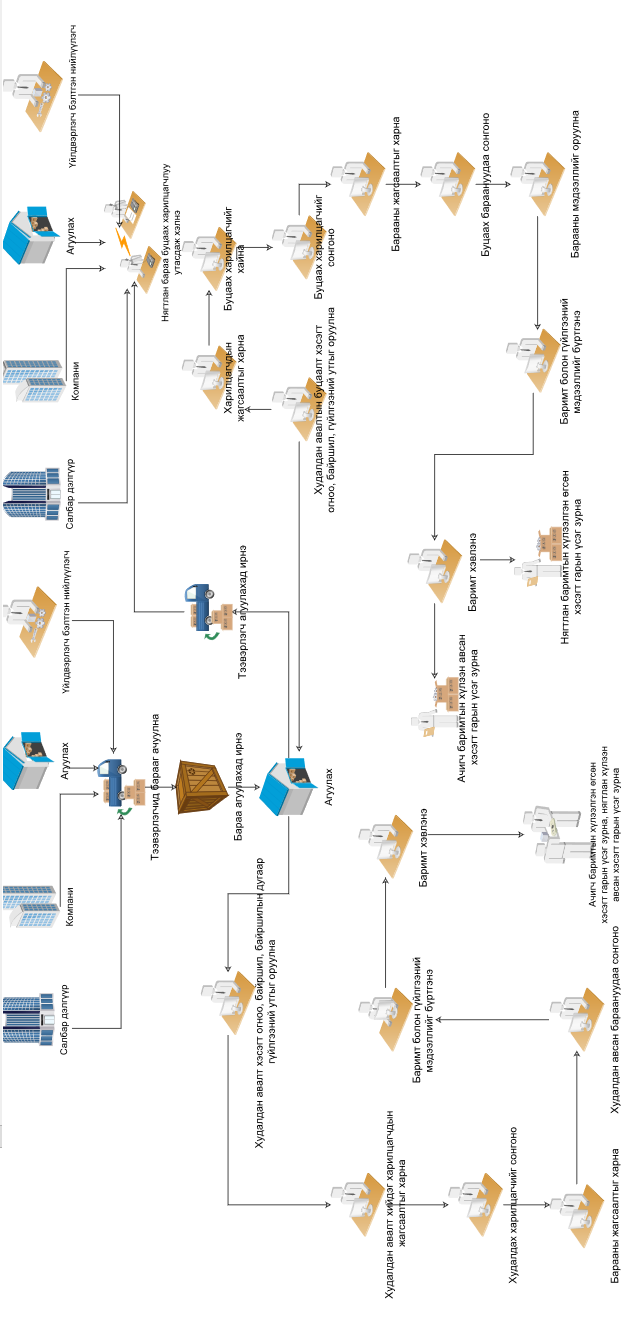
\includegraphics[width=14.5cm, height=20cm]{Diagrams/HudaldanAvWorkFlow2}
	\caption[Худалдан авалтын ажлын урсгал]{Худалдан авалтын ажлын урсгал}
	\label{text}
\end{figure}
\begin{figure}[!h]
	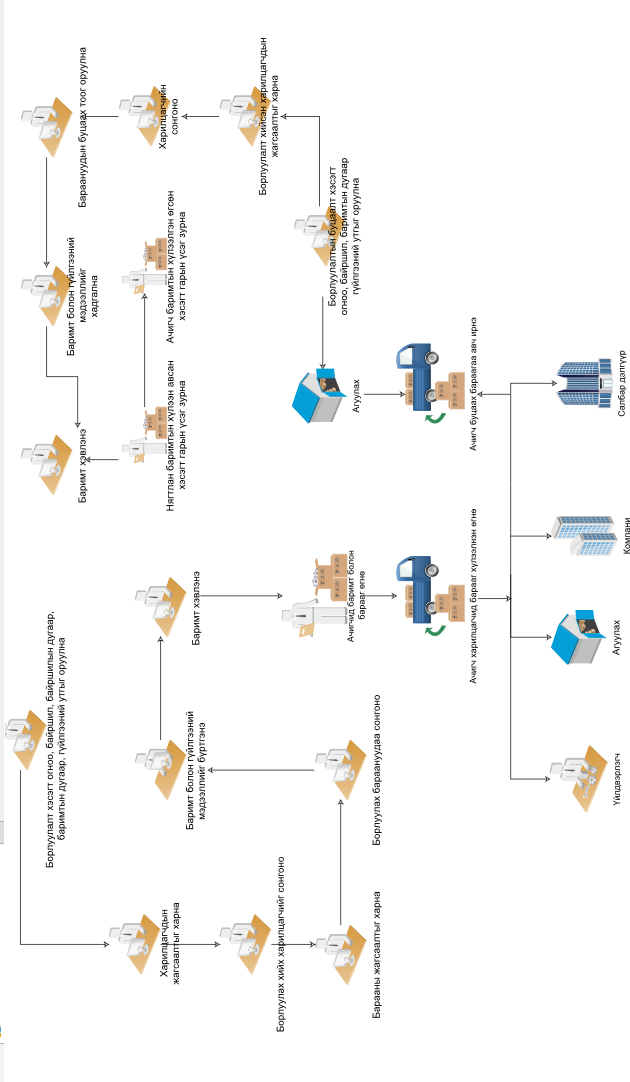
\includegraphics[width=14.5cm, height=20cm]{Diagrams/BorluulaltWorkFlow1}
	\caption[Борлуулалтын ажлын урсгал]{Борлуулалтын ажлын урсгал}
	\label{text}
\end{figure}
\section{Өгөгдлийн ерөнхий схем}
			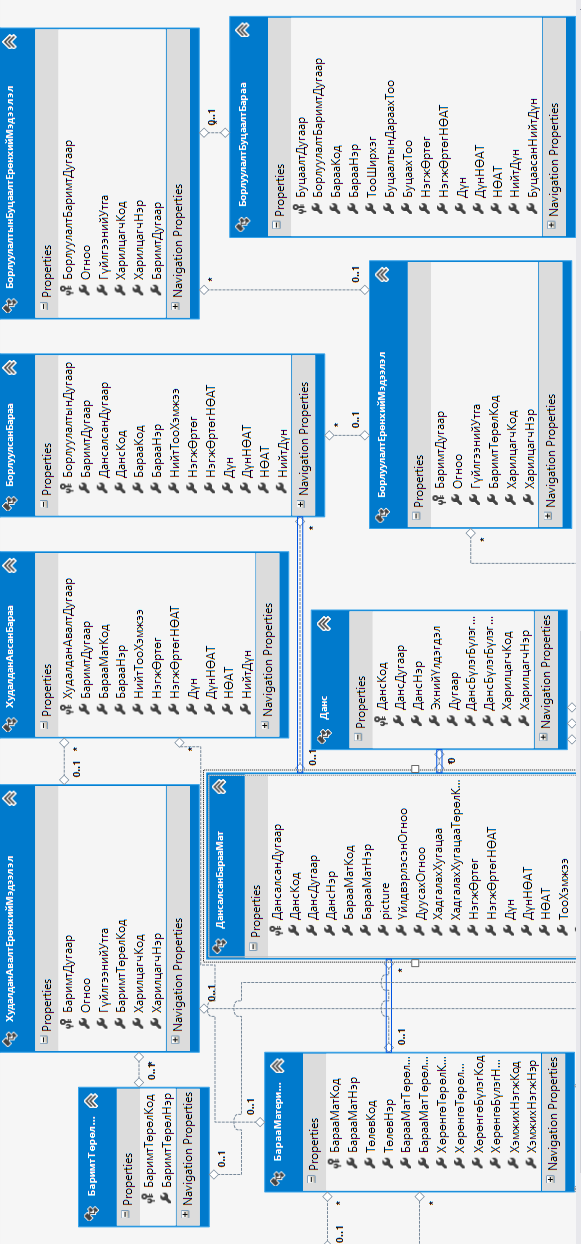
\includegraphics[width=14.5cm,height=22cm]{Diagrams/erd1}
        	\begin{figure}[h!]
        	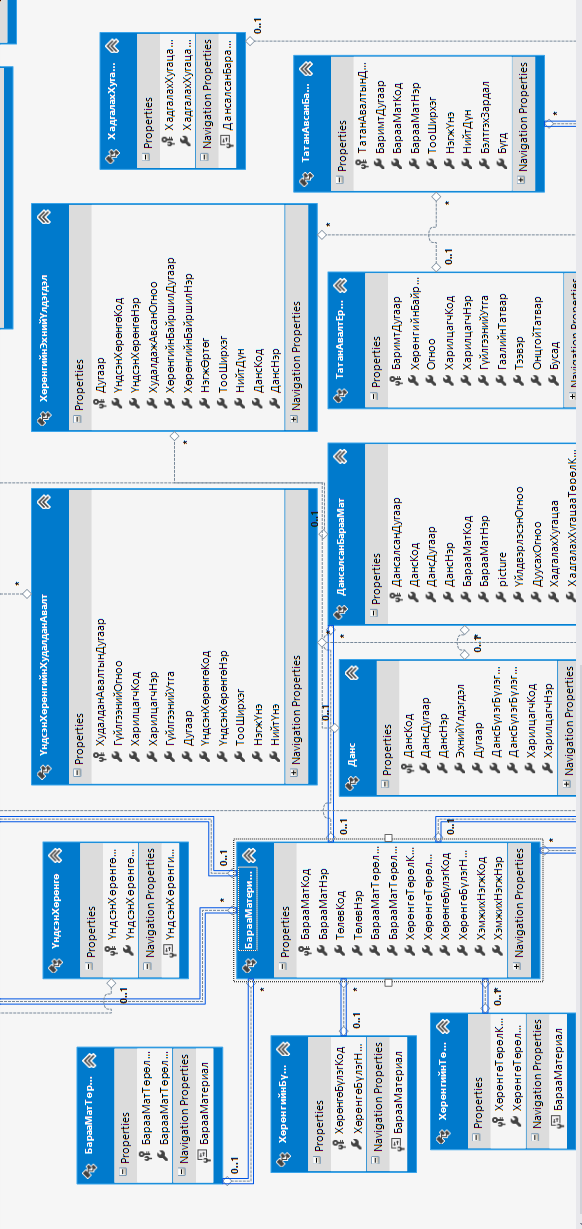
\includegraphics[width=14.5cm,height=21cm]{Diagrams/erd2}
        	\caption[Өгөгдлийн ерөнхий схем]{Өгөгдлийн ерөнхий схем}
        	\label{text}
        \end{figure}
    \vspace*{20in}
\section{Үйл ажиллагааны диаграм}
\begin{figure}[h!]
	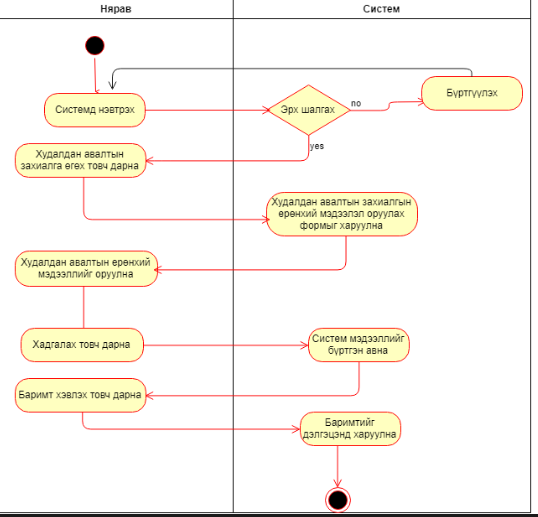
\includegraphics[width=14.5cm, height=14cm]{Diagrams/act2}
	\caption[Худалдан авалт захиалга хийх үйл ажиллагааны диаграм]{Худалдан авалтын  захиалга үйл ажиллагааны диаграм}
	\label{text}
\end{figure}


\begin{figure}[h!]
	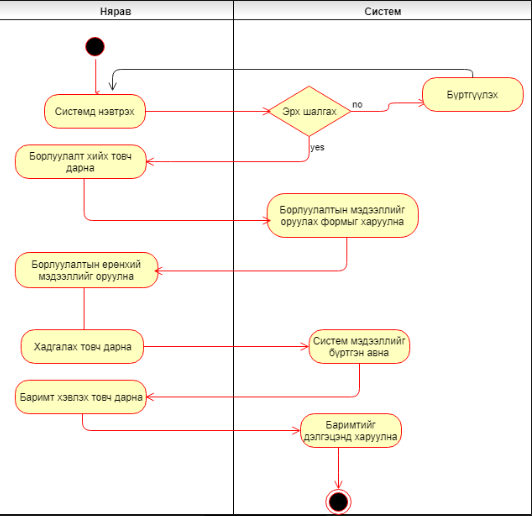
\includegraphics[width=14.5cm, height=14cm]{Diagrams/act3}
	\caption[Борлуулалт хийх үйл ажиллагааны диаграм]{Борлуулалт хийх үйл ажиллагааны диаграм}
	\label{text}
\end{figure}

\begin{figure}[h!]
	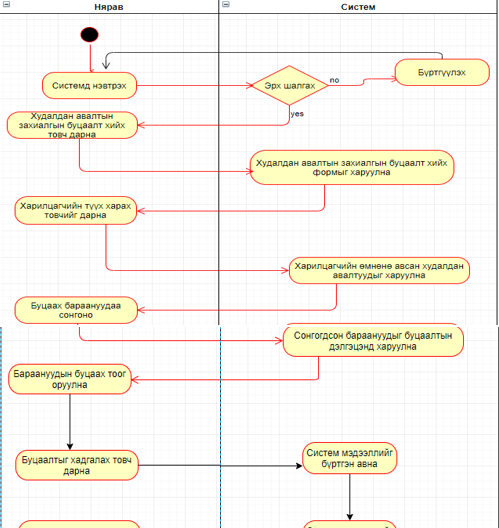
\includegraphics[width=14.5cm, height=22cm]{Diagrams/act4}
	\caption[Худалдан авалтын буцаалтын үйл ажиллагааны диаграм]{Худалдан авалтын буцаалтын үйл ажиллагааны диаграм}
	\label{text}
\end{figure}

 \vspace*{4in}
\section{Класс диаграм}
	\begin{figure}[h!]
		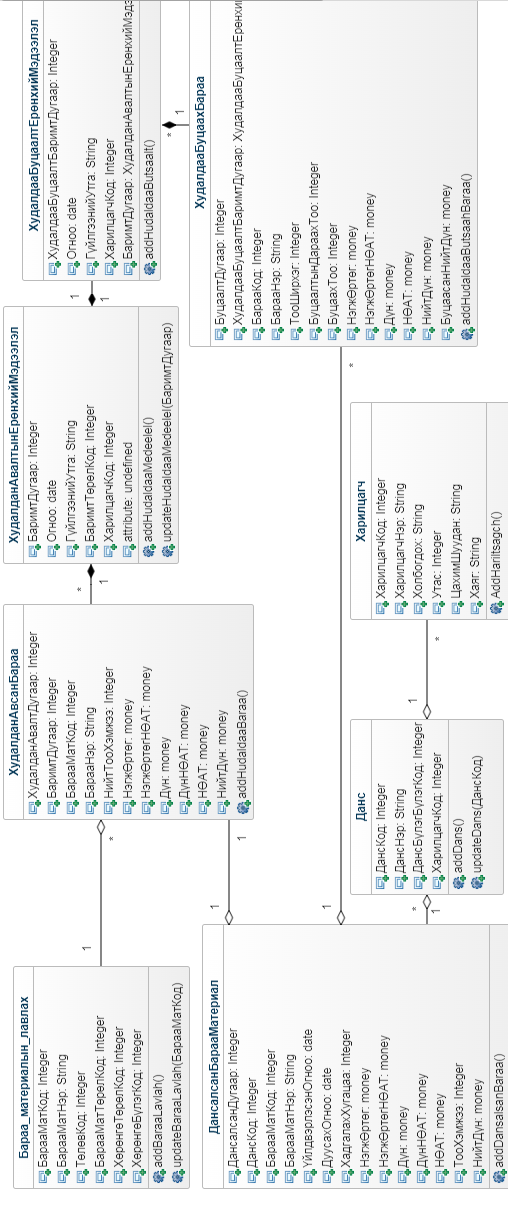
\includegraphics[width=14.5cm, height=20cm]{Diagrams/ka1}
		\caption[Класс диаграм]{Класс диаграм}
		\label{text}
	\end{figure}
	\begin{figure}[h!]
	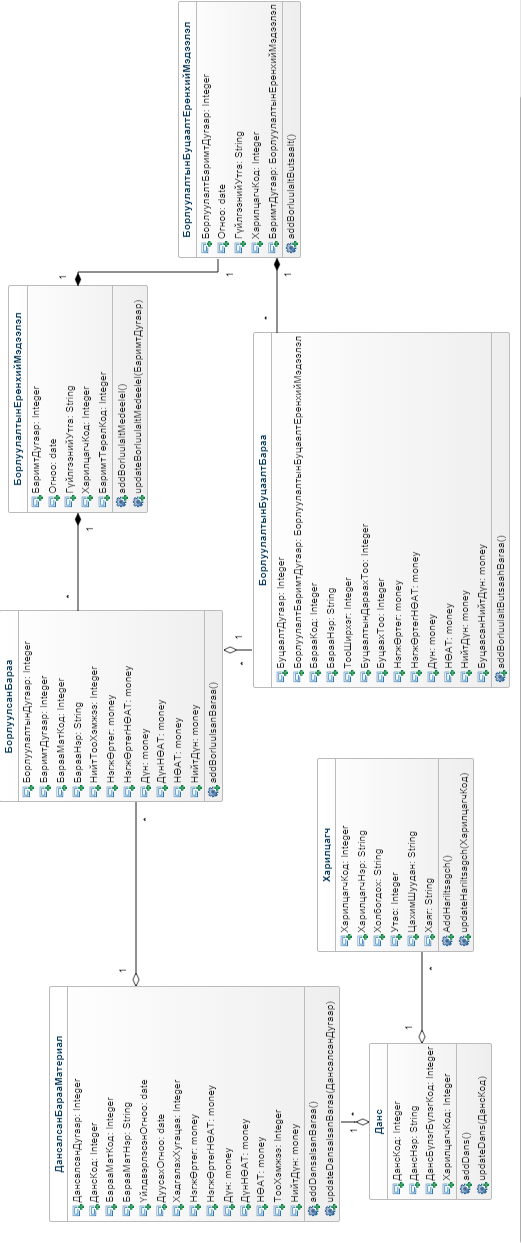
\includegraphics[width=14.5cm, height=22cm]{Diagrams/ka2}
	\caption[Класс диаграм]{Класс диаграм}
	\label{text}
\end{figure}
\section{Дарааллын диаграм }
\begin{figure}[!h]
	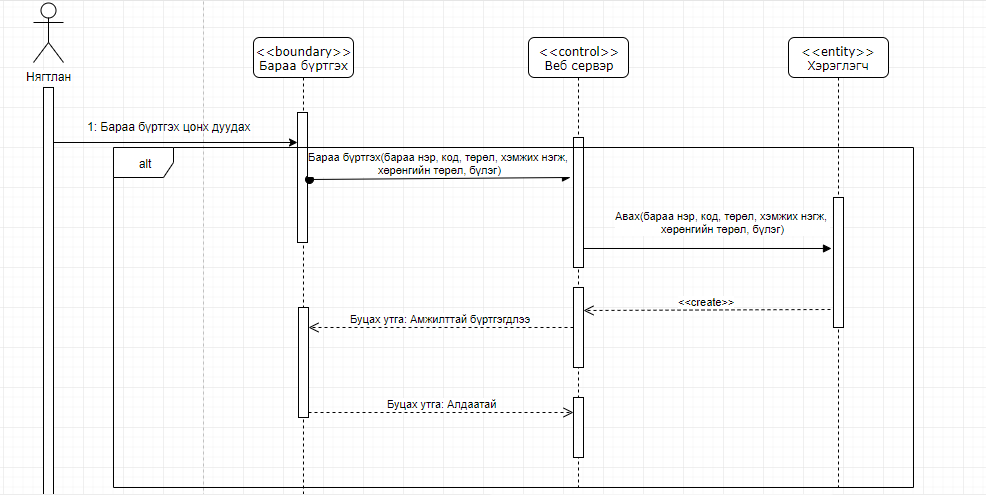
\includegraphics[width=14.5cm, height=10cm]{Diagrams/sec1}
	\caption[Бараа бүртгэх дарааллын диаграм]{Бараа бүртгэх дарааллын диаграм}
	\label{text}
\end{figure}
\section{Төлөвийн диаграм }
\begin{figure}[!h]
	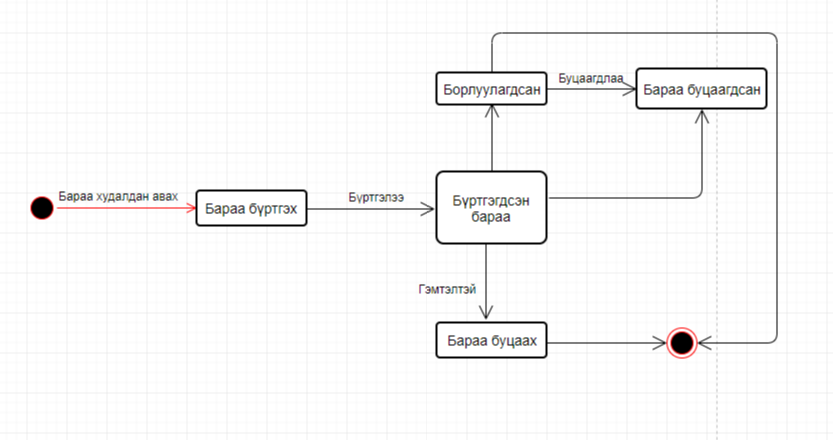
\includegraphics[scale=0.6]{Diagrams/tul2}
	\caption[Төлөвийн диаграм]{Төлвийн диаграм}
	\label{text}
\end{figure}
\section{Дэлгэцийн зохиомж}
\begin{figure}[!h]
	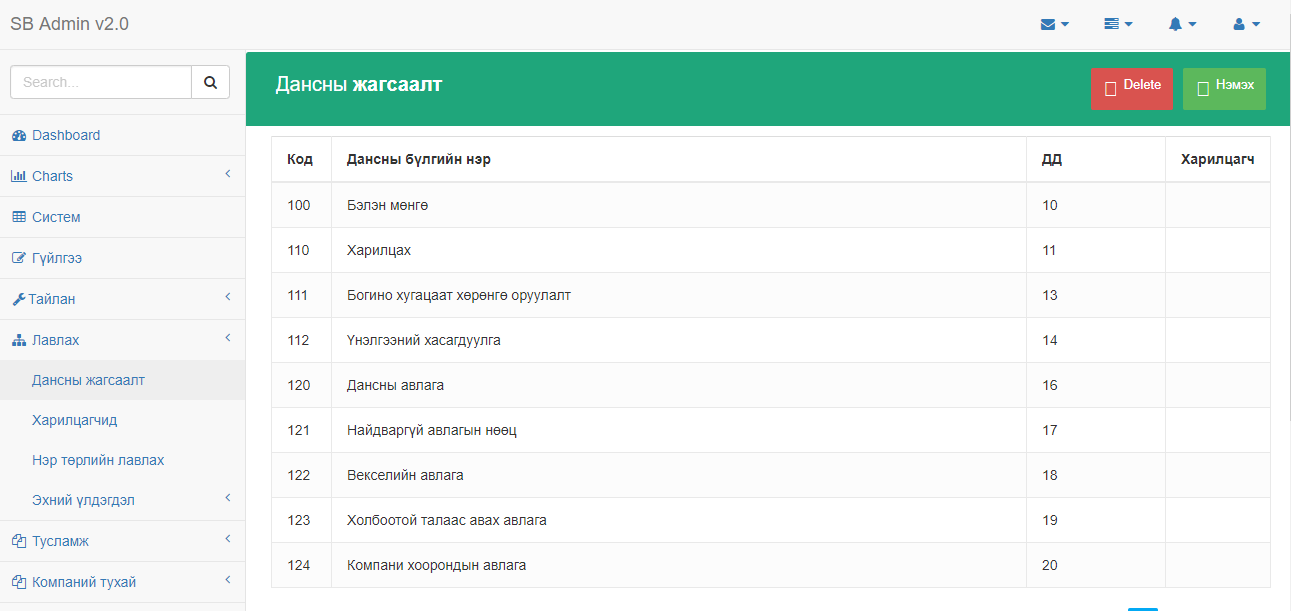
\includegraphics[width=14.5cm, height=10cm]{Diagrams/de1}
	\caption[Нягтлан: Дансны жагсаалт]{Нягтлан: Дансны жагсаалт}
	\label{text}
\end{figure}
\begin{figure}[!h]
	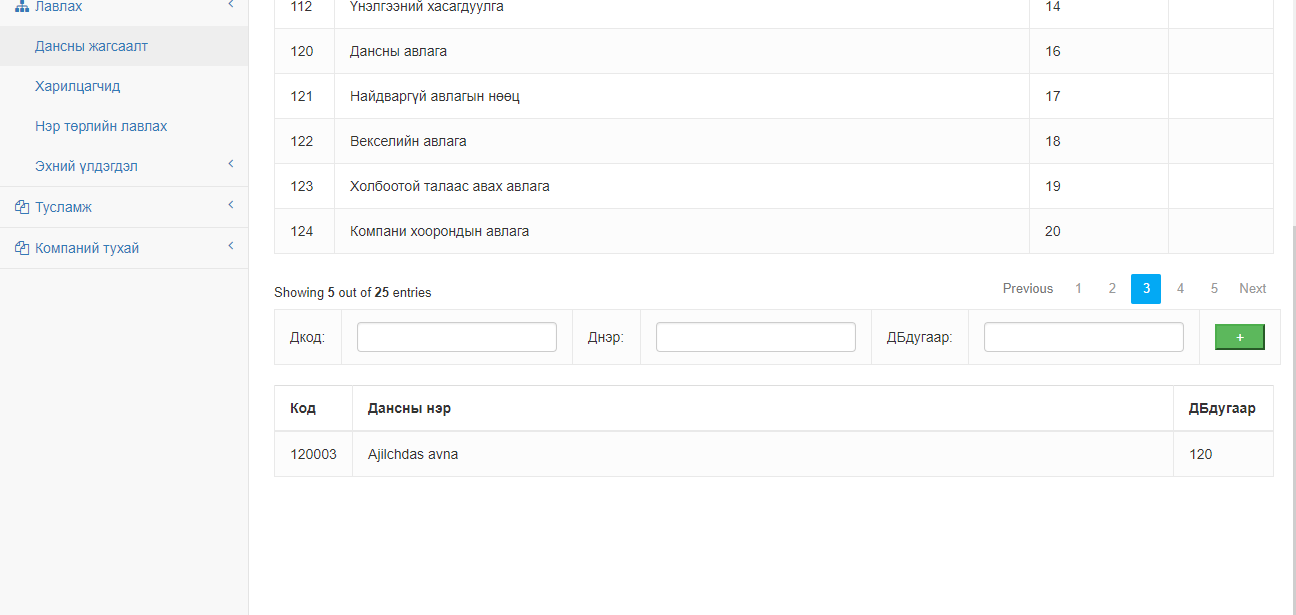
\includegraphics[width=14.5cm, height=9cm]{Diagrams/de2}
	\caption[Нягтлан: Данс бүртгэх]{Нягтлан: Данс бүртгэх}
	\label{text}
\end{figure}
\begin{figure}[!h]
	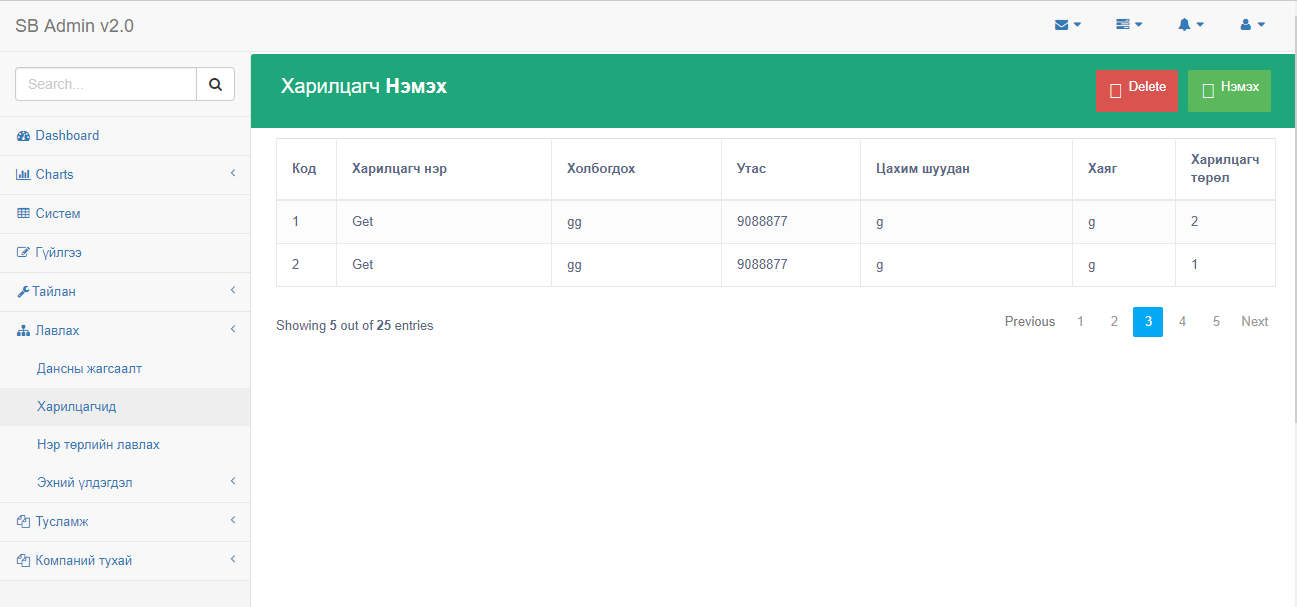
\includegraphics[width=14.5cm, height=10cm]{Diagrams/de3}
	\caption[Нягтлан: Харилцагчдын жагсаалт]{Нягтлан: Харилцагчдын жагсаалт}
	\label{text}
\end{figure}
\begin{figure}[!h]
	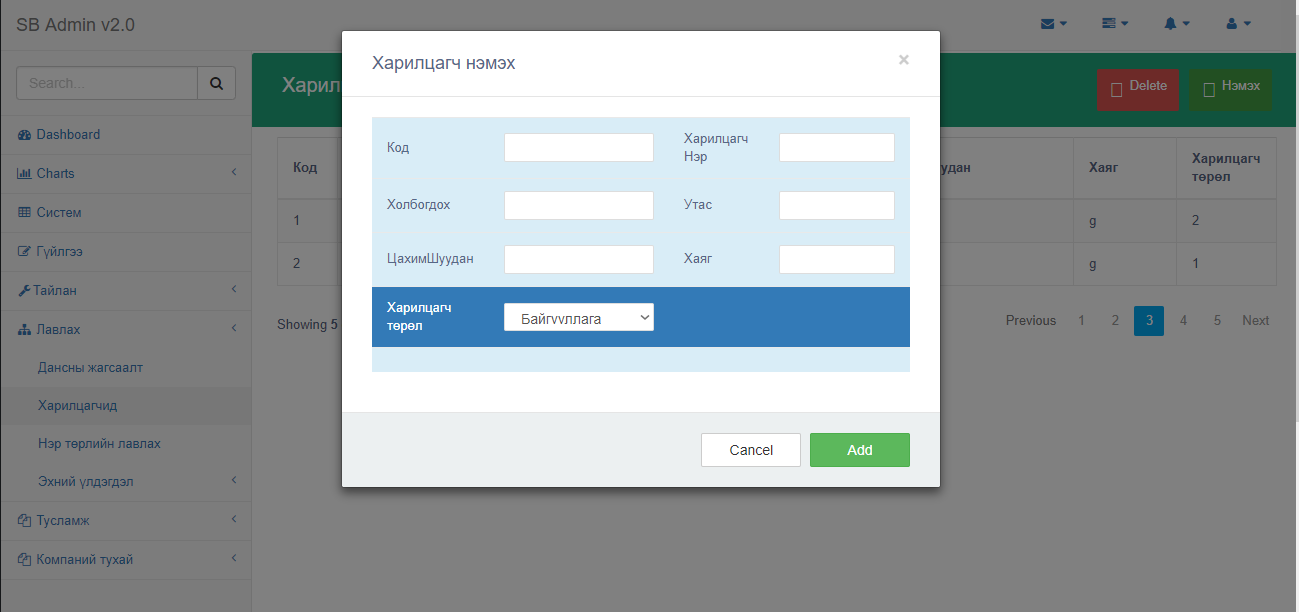
\includegraphics[width=14.5cm, height=11cm]{Diagrams/de4}
	\caption[Нягтлан: Харилцагч бүртгэх]{Нягтлан: Харилцагч бүртгэх}
	\label{text}
\end{figure}
\begin{figure}[!h]
	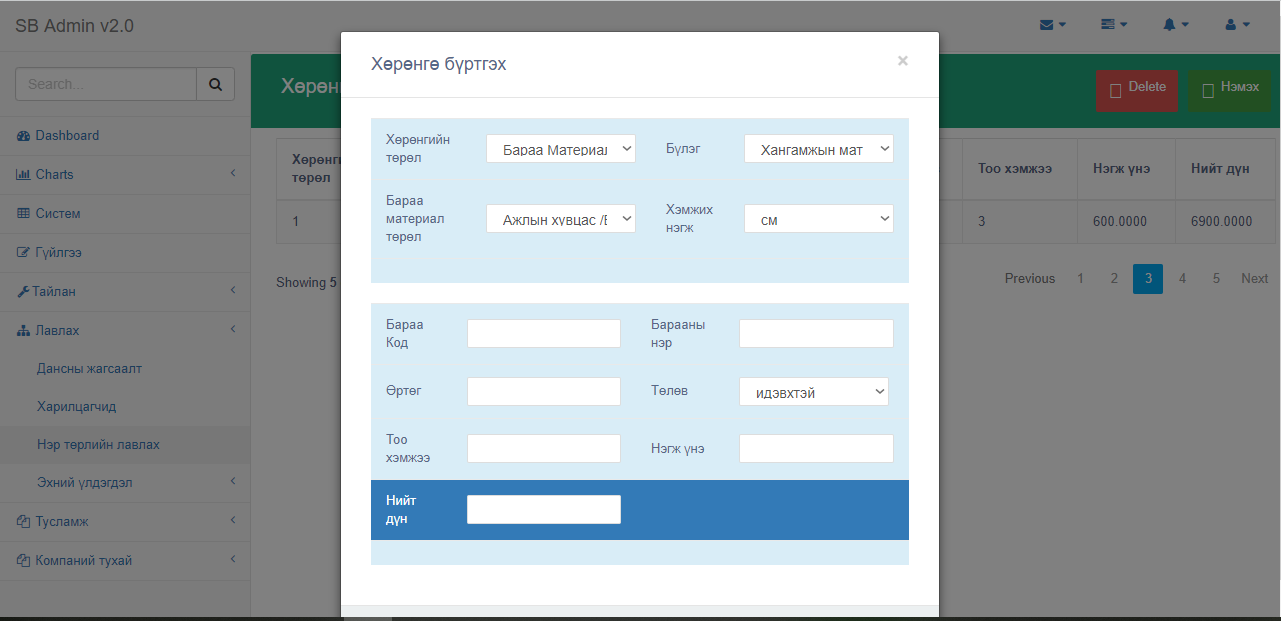
\includegraphics[width=14.5cm, height=11cm]{Diagrams/de6}
	\caption[Нягтлан: Хөрөнгө бүртгэх]{Нягтлан: Хөрөнгө бүртгэх}
	\label{text}
\end{figure}
\begin{figure}[!h]
	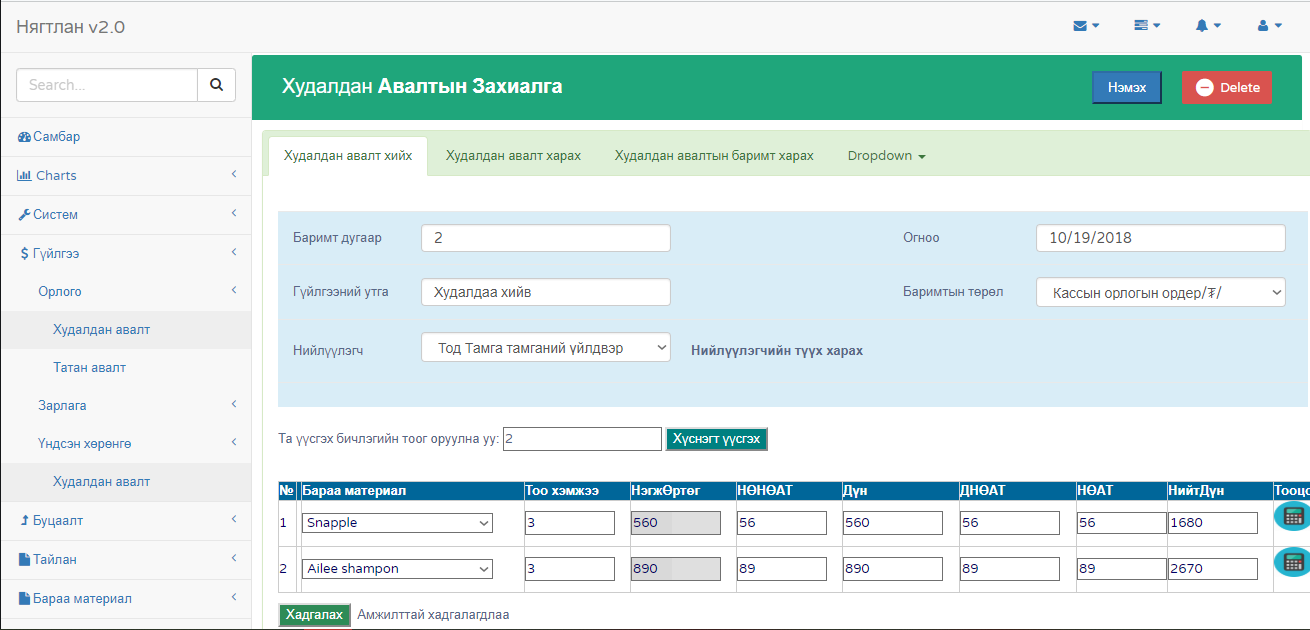
\includegraphics[width=14.5cm, height=10cm]{Diagrams/ke1}
	\caption[Нягтлан: Худалдан авалтын захиалга хийх]{Нягтлан: Худалдан авалт захиалга хийх}
	\label{text}
\end{figure}
\begin{figure}[!h]
	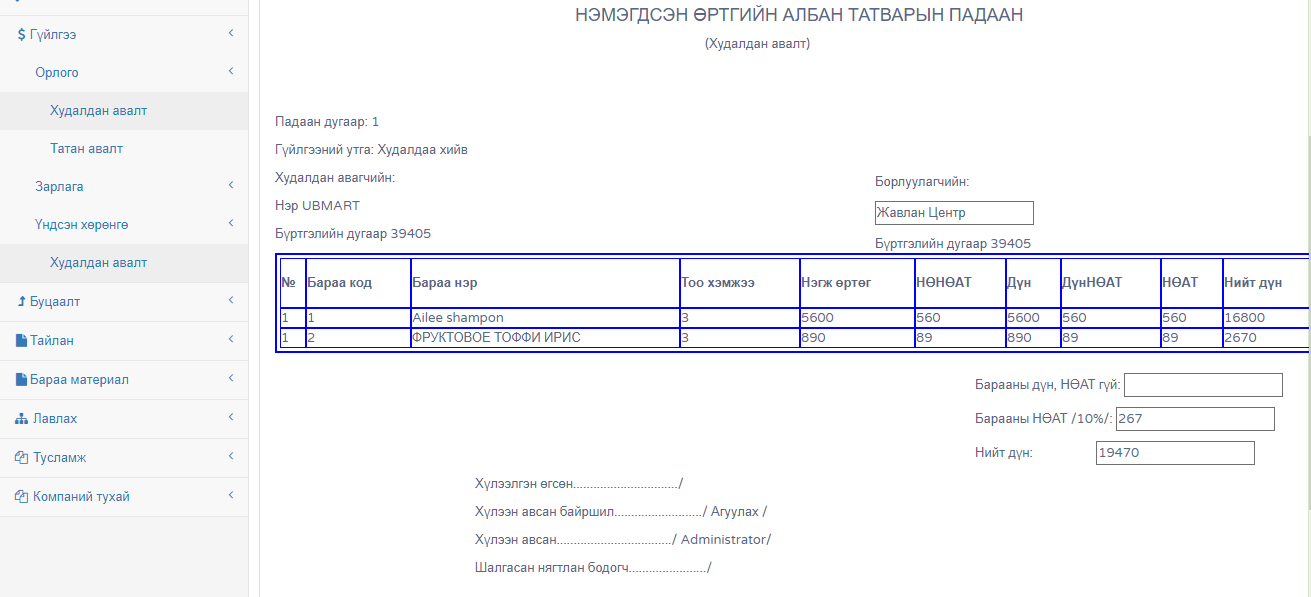
\includegraphics[width=14.5cm, height=10cm]{Diagrams/ke2}
	\caption[Нягтлан: Худалдан авалтын баримт харах]{Нягтлан: Худалдан авалтын баримт хэвлэх}
	\label{text}
\end{figure}
\begin{figure}[!h]
	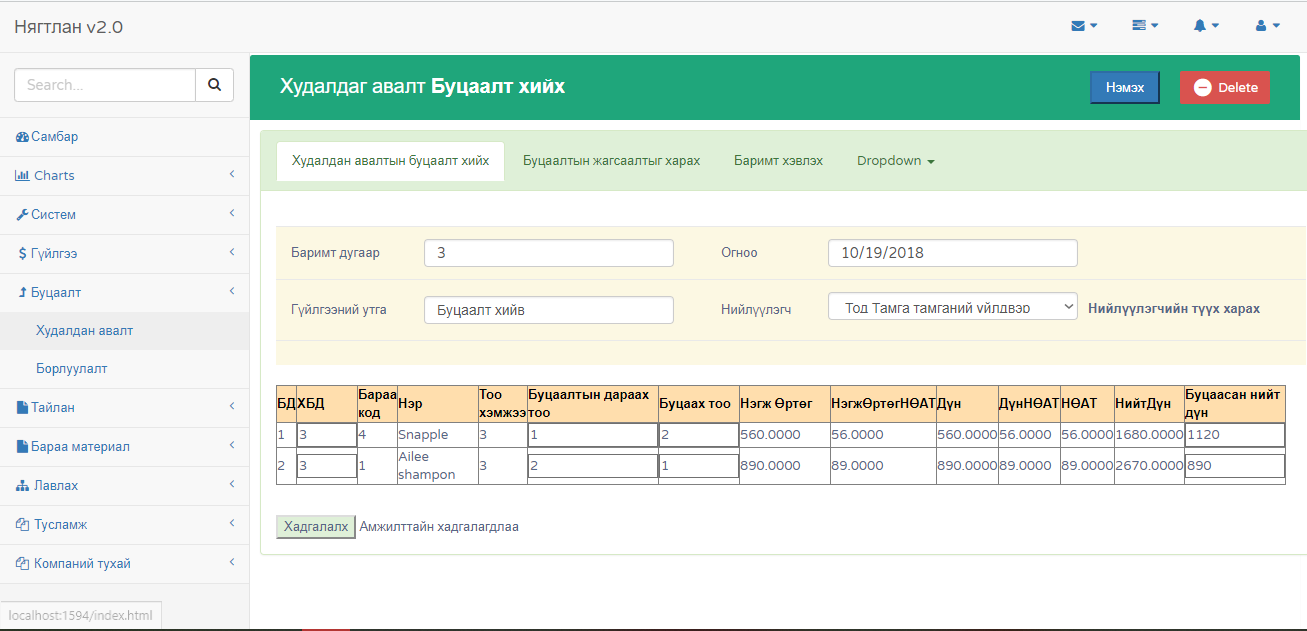
\includegraphics[width=14.5cm, height=10cm]{Diagrams/ke3}
	\caption[Нягтлан: Худалдан авалтын захиалгын буцаалт хийх]{Нягтлан:Худалдан авалтын захиалгын буцаалт хийх}
	\label{text}
\end{figure}
\begin{figure}[!h]
	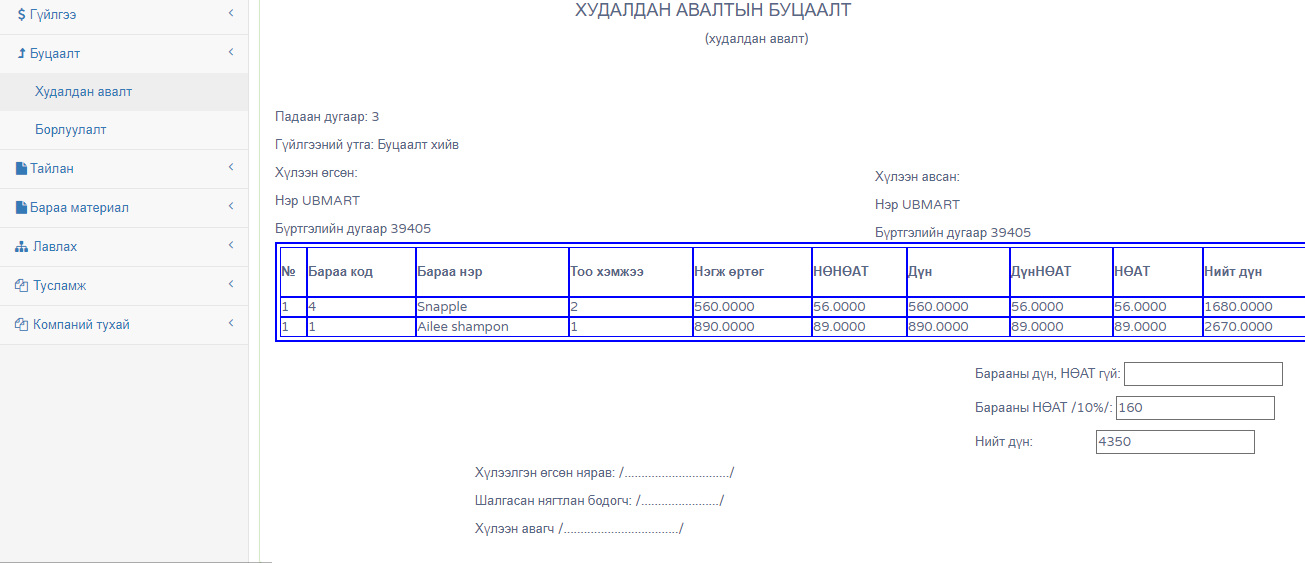
\includegraphics[width=14.5cm, height=10cm]{Diagrams/ke4}
	\caption[Нягтлан: Худалдан авалтын буцаалт баримт хэвлэх]{Нягтлан:Худалдан авалтын буцаалтын баримт хэвлэх}
	\label{text}
\end{figure}
\begin{figure}[!h]
	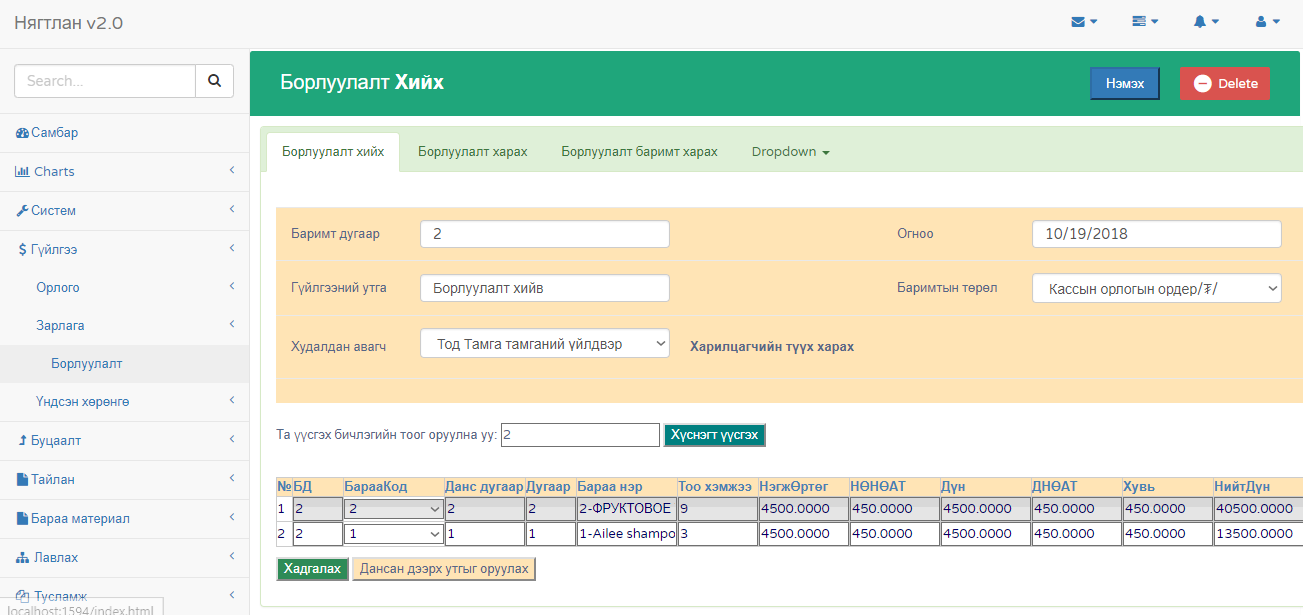
\includegraphics[width=14.5cm, height=10cm]{Diagrams/ke5}
	\caption[Нягтлан: Борлуулалт хийх]{Нягтлан:Борлуулалт хийх}
	\label{text}
\end{figure}
\begin{figure}[!h]
	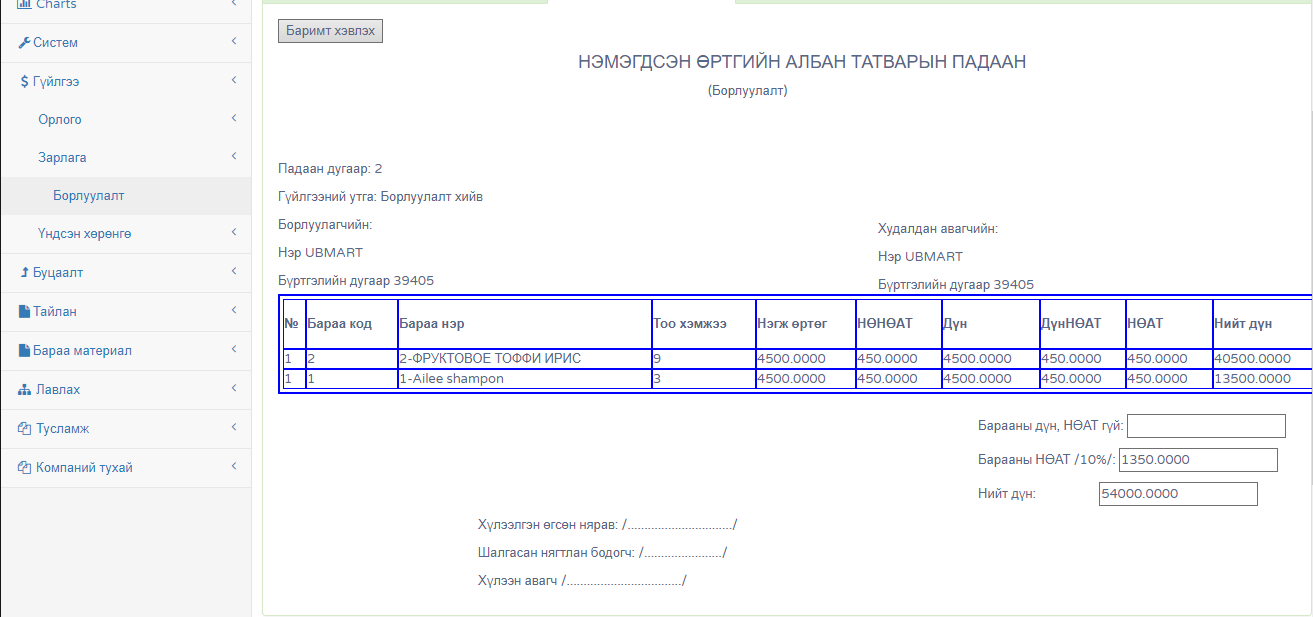
\includegraphics[width=14.5cm, height=10cm]{Diagrams/ke6}
	\caption[Нягтлан: Борлуулалт баримт хэвлэх]{Нягтлан:Борлуулалт баримт хэвлэх}
	\label{text}
\end{figure}
\begin{figure}[!h]
	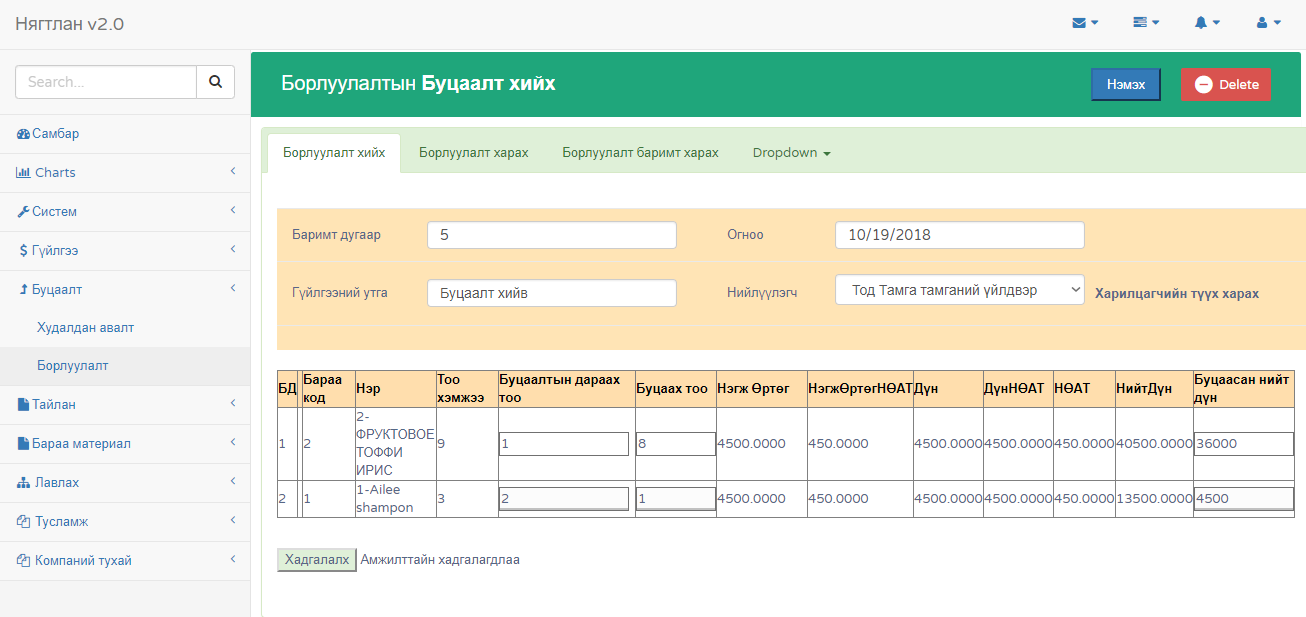
\includegraphics[width=14.5cm, height=11cm]{Diagrams/ke7}
	\caption[Нягтлан: Борлуулалтын буцаалт хийх]{Нягтлан:Борлуулалтын буцаалт  хийх}
	\label{text}
\end{figure}
\begin{figure}[!h]
	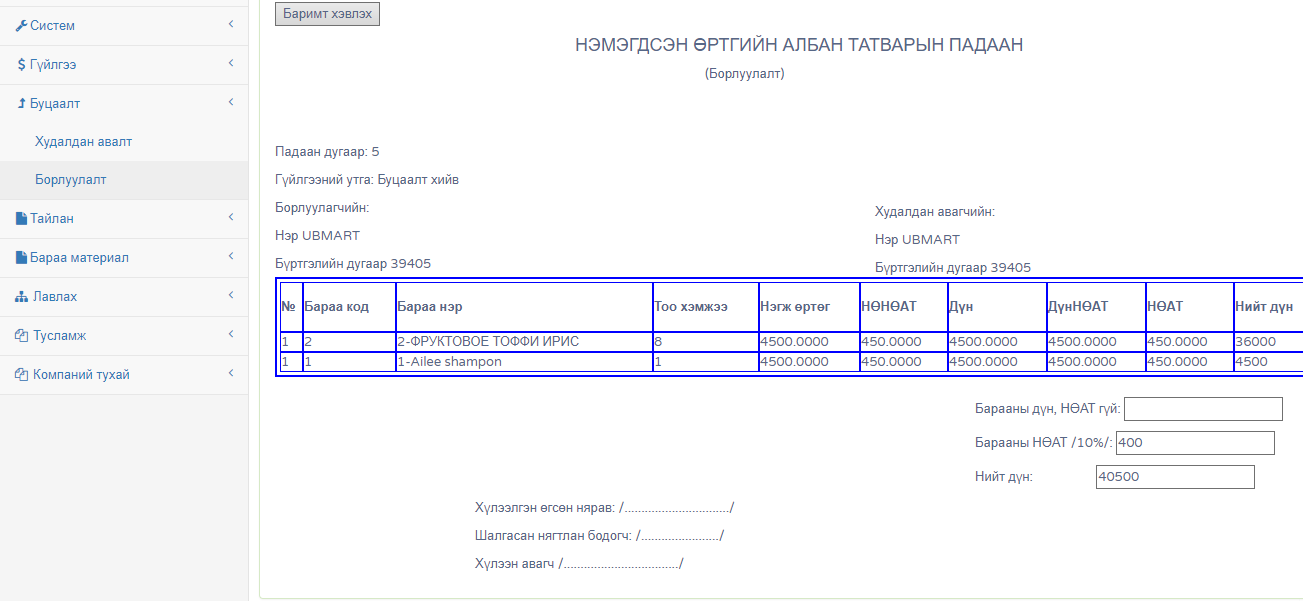
\includegraphics[width=14.5cm, height=10cm]{Diagrams/ke8}
	\caption[Нягтлан: Борлуулалтын буцаалт баримт хэвлэх]{Нягтлан:Борлуулалтын буцаалтын баримт хэвлэх}
	\label{text}
\end{figure}
\begin{figure}[!h]
	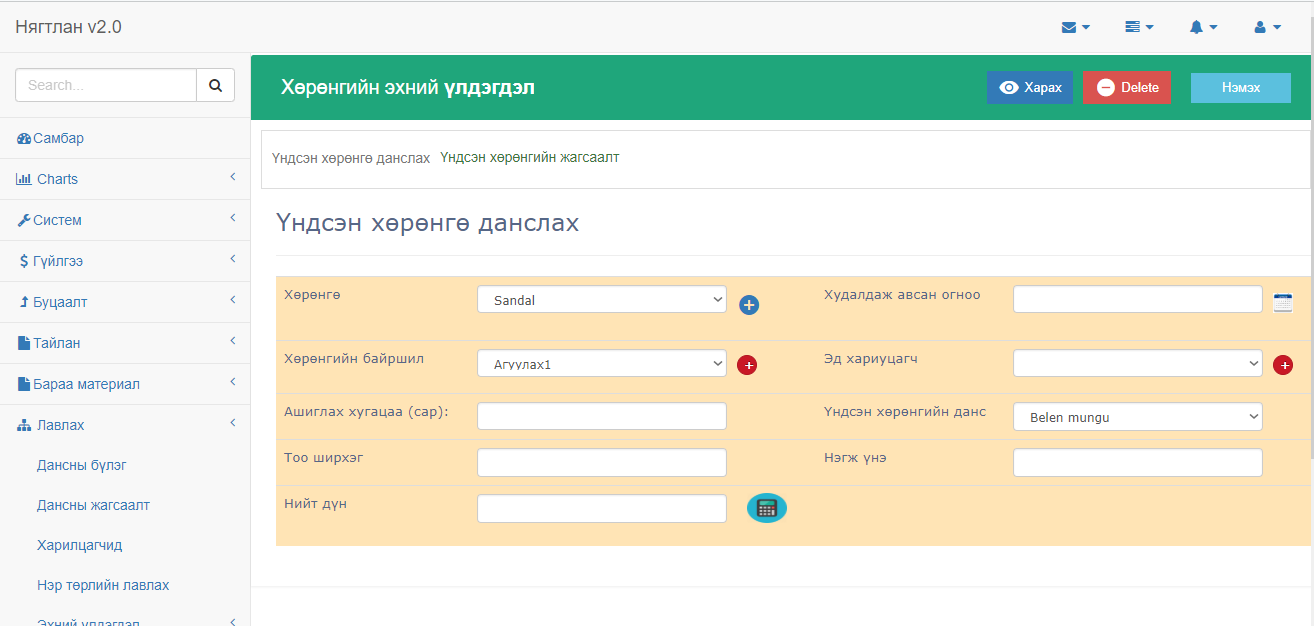
\includegraphics[width=14.5cm, height=11cm]{Diagrams/ke9}
	\caption[Нягтлан: Үндсэн хөрөнгө данслах]{Нягтлан:Үндсэн хөрөнгө данслах}
	\label{text}
\end{figure}
\begin{figure}[!h]
	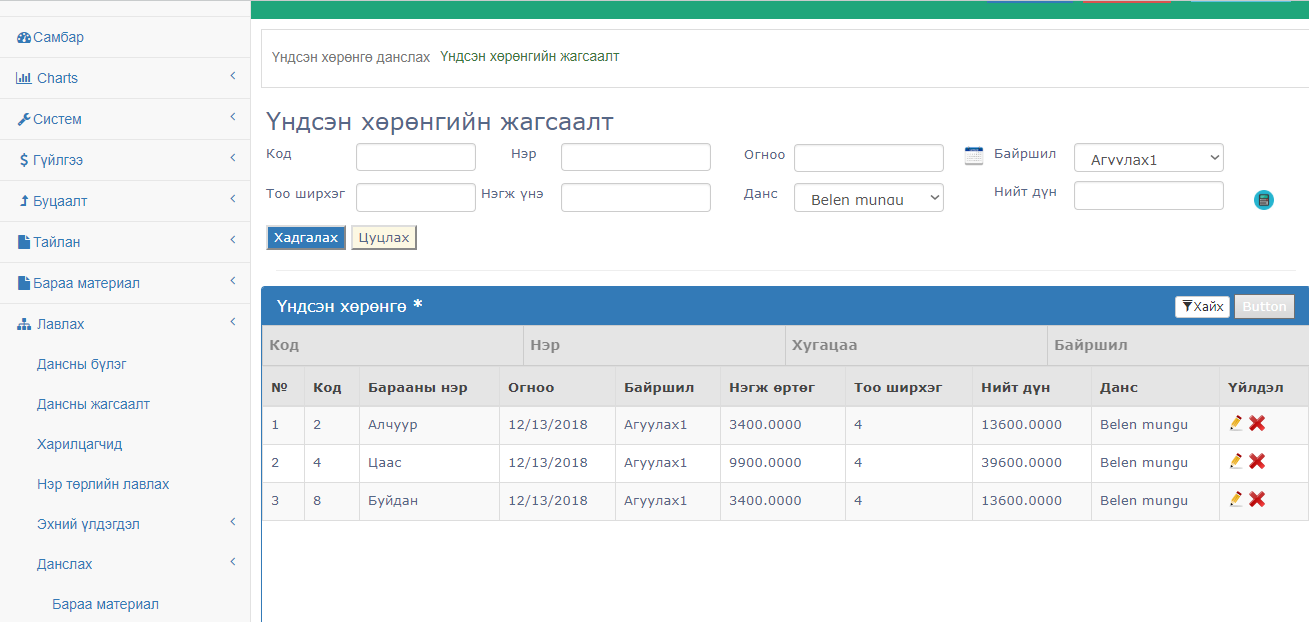
\includegraphics[width=14.5cm, height=10cm]{Diagrams/ke10}
	\caption[Нягтлан: Үндсэн хөрөнгийн жагсаалт]{Нягтлан:Үндсэн хөрөнгийн жагсаалт}
	\label{text}
\end{figure}
\begin{figure}[!h]
	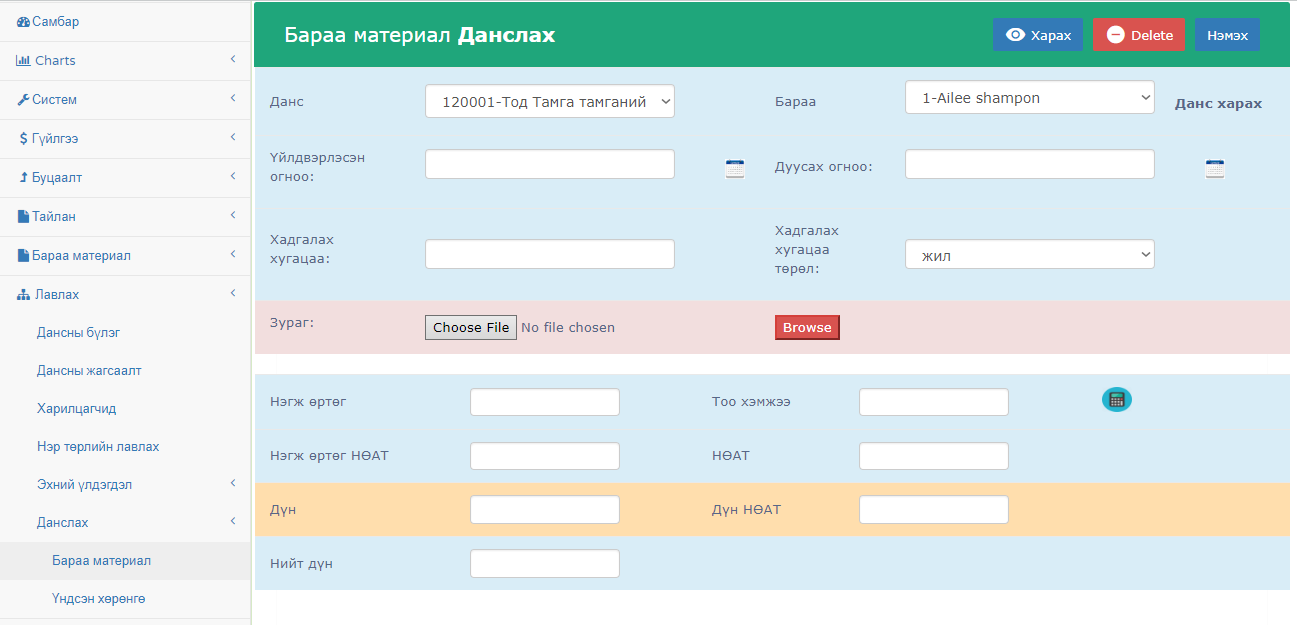
\includegraphics[width=14.5cm, height=11cm]{Diagrams/ke11}
	\caption[Нягтлан: Бараа материал данслах]{Нягтлан:Бараа материал данслах}
	\label{text}
\end{figure}
\begin{figure}[!h]
	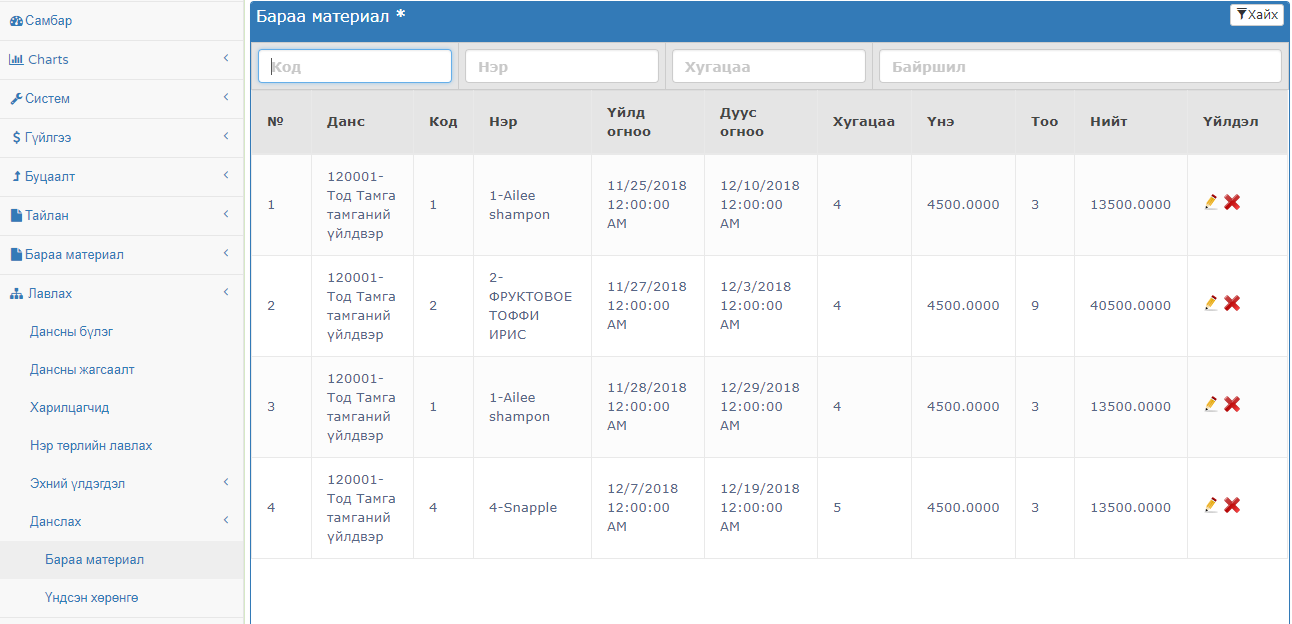
\includegraphics[width=14.5cm, height=10cm]{Diagrams/ke12}
	\caption[Нягтлан: Бараа материалын жагсаалт]{Нягтлан:Бараа материалын жагсаалт}
	\label{text}
\end{figure}
\begin{figure}[!h]
	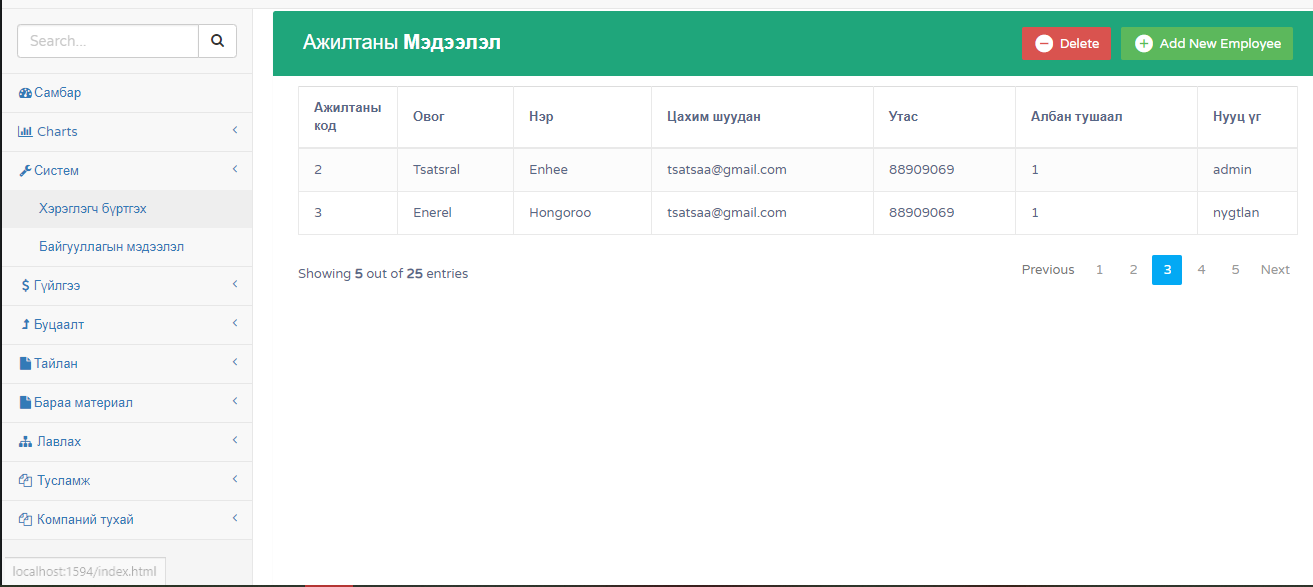
\includegraphics[width=14.5cm, height=11cm]{Diagrams/ke13}
	\caption[Админ: Хэрэглэгч нэмэх]{Админ: Хэрэглэгч нэмэх}
	\label{text}
\end{figure}
\section{Тайлан, статистик үзүүлэлтийн загвар }
\begin{figure}[!h]
	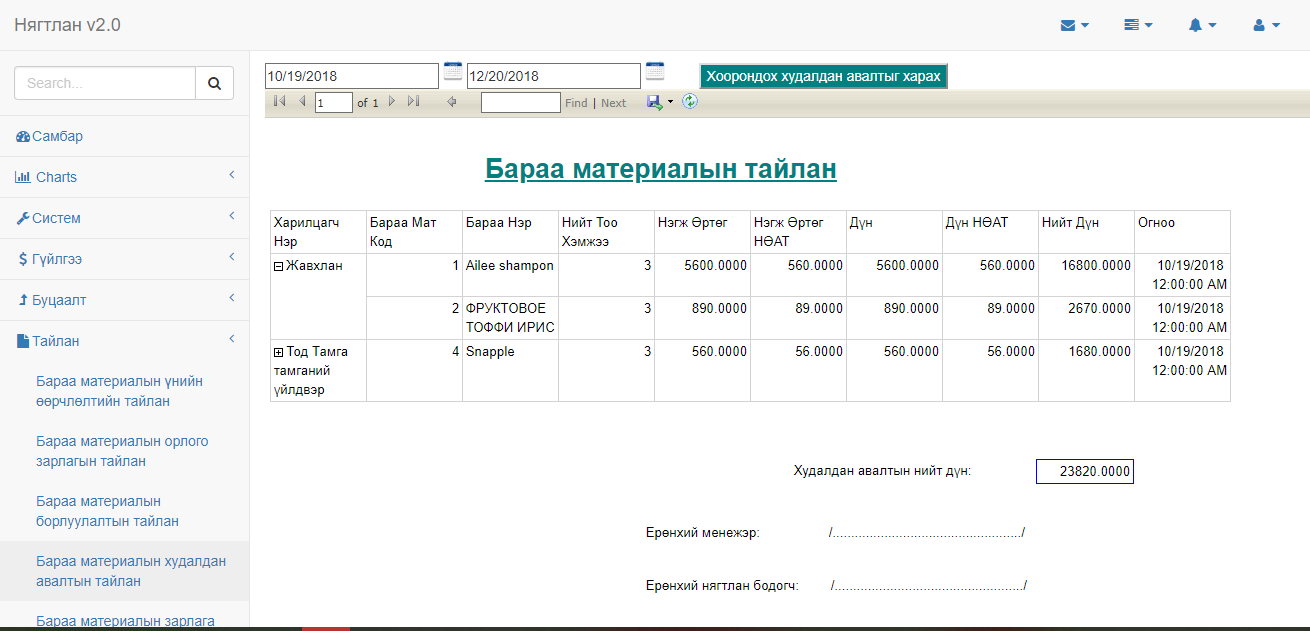
\includegraphics[width=14.5cm, height=10cm]{Diagrams/ce1}
	\caption[Нягтлан: Худалдан авалтын тайлан]{Нягтлан: Худалдан авалтын тайлан}
	\label{text}
\end{figure}
\begin{figure}[!h]
	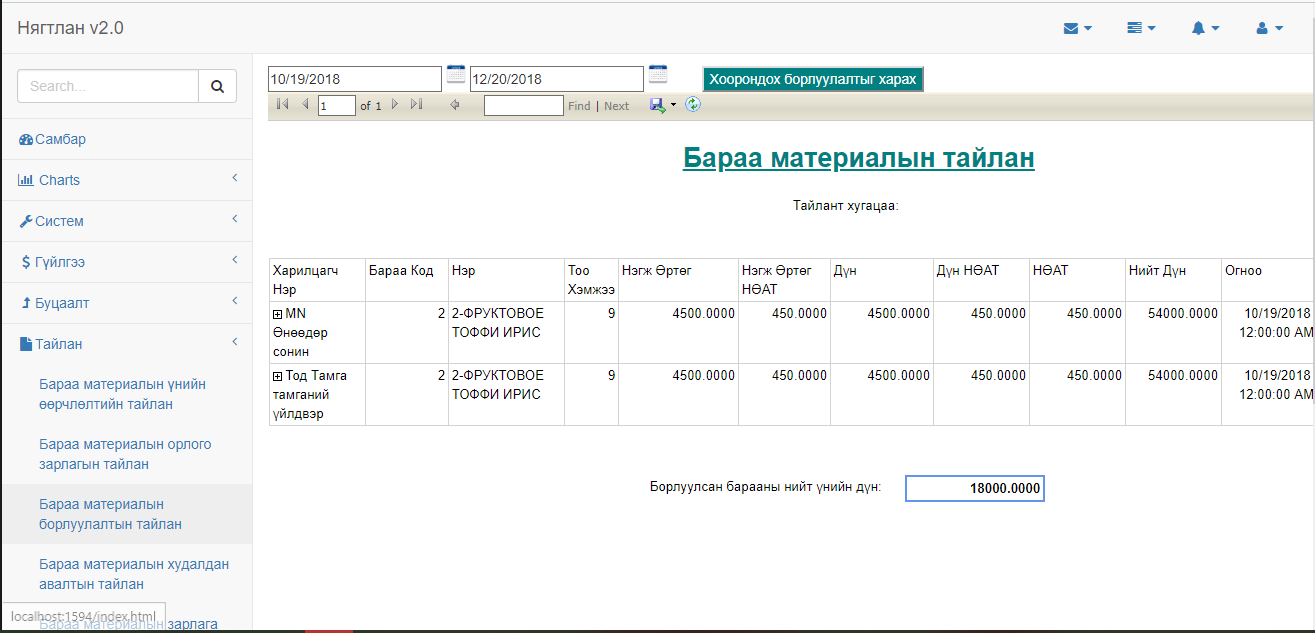
\includegraphics[width=14.5cm, height=9cm]{Diagrams/ce2}
	\caption[Нягтлан: Борлуулалтын тайлан]{Нягтлан: Борлуулалтын тайлан}
	\label{text}
\end{figure}
\section{Ерөнхий дүгнэлт}
\qquad Өнөө үед интернэтийн орчинд ажил, үйлчилгээгээ явуулах хувь хүн болон аж ахуйн нэгж албан байгууллагууд хурдацтай өсөн нэмэгдсэн билээ. Үүнийг ажиглан агуулахын 
системийг байгууллагад хүргэх нь одоогийн нийгэмд хамгийн зөв арга хэлбэр. Энэхүү системийг хийхэд дараах ажлуудыг хийж гүйцэтгэлээ:

-	Тухайн системийн талаар судалгаа явсан

-	Өгөгдлийн сан болон вебийн дотоод үйл ажиллагааг дүрслэн гаргасан

-	Код бичих орчиноо бэлдэх, судалгаа шинжилгээ хийсэн










	

	
	
